% $Id: CONTENT.tex 11058 2010-05-06 14:44:53Z alexandra $
% Local Variables:
% ispell-check-comments: nil
% Local IspellDict: american
% End:
% --------------------------------------------------------
% User documentation
% copyright by BREDEX GmbH 2004
% --------------------------------------------------------

Open the \jb{} preferences dialog (\bxfigref{gdprefs}) by selecting:\\
\bxmenu{Window}{Preferences}{}.

\subsection{\jb{}{} preferences}
\gdhelpid{prefPageBasicContextId}{GUIdancer Preferences}
% $Id: gdprefs.tex 11355 2010-06-16 14:48:31Z alexandra $
%ID:prefPageBasicContextId
% Local Variables:
% ispell-check-comments: nil
% Local IspellDict: american
% End:
% --------------------------------------------------------
% User documentation
% copyright by BREDEX GmbH 2004
% --------------------------------------------------------
\index{Preferences!Test}
\index{Test!Preferences}
\label{gdprefs}

\begin{figure}[h]
\begin{center}
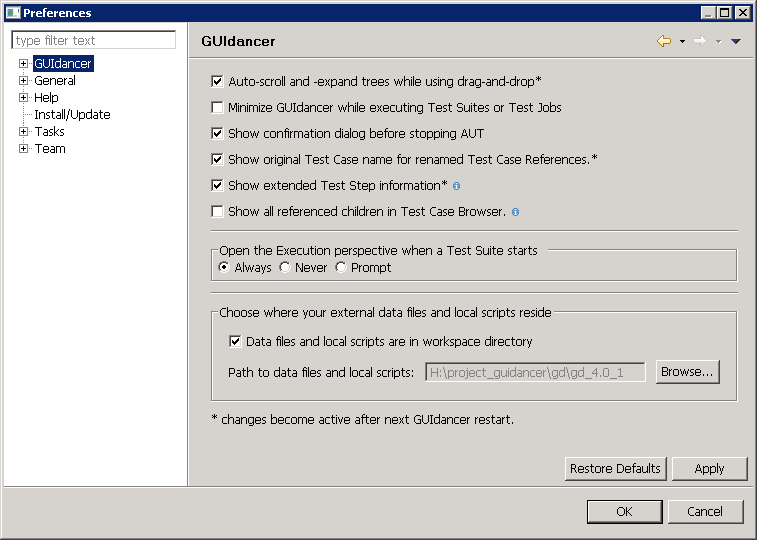
\includegraphics[width=0.60\textwidth]{Tasks/Preferences/PS/gdprefs}
\caption{Preference Dialog}
\label{gdprefs}
\end{center}
\end{figure}

 In the preferences dialog, select \bxname{Test} from the tree on the left hand side.

From this page, you can configure your preferences for:
\begin{description}
\item [Auto-scrolling and -expanding:]{When the checkbox is marked, the views and browsers  automatically scroll in the direction you move the mouse when you are dragging and dropping. Trees will also be automatically expanded when you hover over them while dragging items.}
\item [Minimizing the \ite{}:]{When the checkbox is marked, the \ite{} is automatically minimized when test execution begins. This is useful if you are letting tests run on the same machine you are specifying on.}
\item [\gdaut{} confirmation dialog:]{When the checkbox is marked, a dialog appears to check if you are sure when you click the  \bxcaption{stop \gdaut{}} button.}
\item [Original \gdcase{} name:]{When the checkbox is activated, you can see the original name of a referenced \gdcase{} in brackets behind a new name you enter for the \gdcase{}. This can help you to see and search for \gdcases{} you have reused. }
\item[\gdstep{} information:]{When this checkbox is activated, you see the details about the \gdstep{} (the component name and type, and the action) in square brackets behind the \gdstep{} name. If you do not want to see these details, you can deactivate this checkbox.}
\item[Show referenced children:]{When this option is not active, you can only see  referenced parent \gdcases{} in the \gdtestcasebrowser{}. The referenced \gdcases{} contained in these \gdcases{} are not displayed. This action can be useful if you want to improve the speed of working with the \ite{}.}
\item [\gdproject{} auto load:]{If you have selected a \gdproject{} to be automatically loaded \bxpref{TasksAutoLoadProject}, then you can stop the auto-loading by deactivating the checkbox.}
\item [Switching to the \execpersp{}:]{When the test begins, the \ite{} can automatically change to the \execpersp{}. You can choose to always be asked, to always change, or to never change. }
\item [Data files location:]{You can specify a location where external data files (e.g. Excel files) are held, or use the workspace directory as the base location. }
\bxtipp{The advantage of using the workspace as a location for your data files is that you can view these in the navigator view directly in the \ite{}. Windows users can even open Excel files from the \ite{} using the In-Place editor.}
\end{description}

 



\subsection{Appearance preferences}
\gdhelpid{appearancePrefPageContextId}{Appearance Preferences}
\index{Modeling!Appearance}
\index{Appearance!Model}

There are various ways of altering the appearance of the model and the canvas. 

In the main menu, under the \bxname{Modeling} menu, you can alter details about the fonts, colors and lines as well as choosing whether to show grids and rulers. These options are also available in the \gdpropview{} in the modeling perspective under the \bxname{Appearance} and \bxname{Rulers \& Grid} tabs. 

You can also set appearance features in the preferences for modeling \bxpref{TasksPrefsModel}. 


\subsection{\gdserver preferences}
\gdhelpid{prefPageServerContextId}{AUT Agent Preferences}
\gdhelpid{autConfigPropDialogContextId}{Adding/editing AUT configurations}
\gdhelpid{autConfigSettingWizardPagePageContextId}{Configuring an AUT}
% $Id: serverConfigPrefPage.tex 10532 2010-03-16 15:57:20Z alexandra $
% Local Variables:
% ispell-check-comments: nil
% Local IspellDict: american
% End:
% --------------------------------------------------------
% User documentation
% copyright by BREDEX GmbH 2004
% --------------------------------------------------------

\label{serverConfigPrefPage}
\index{Preferences!AUT Agent}
\index{AUT Agent!Preferences}
\index{Add!AUT Agent}
\index{AUT Agent!Add}


\begin{enumerate}
\item In the \gdagent{} preference page, you can add, edit and delete \gdagent{}s and port numbers. 
\bxtipp{The \gdagent preference page can also be accessed from the \gdaut{} configuration dialog which you can open from the \gdproject{} properties.}
\end{enumerate}




\begin{figure}[p]
\begin{center}
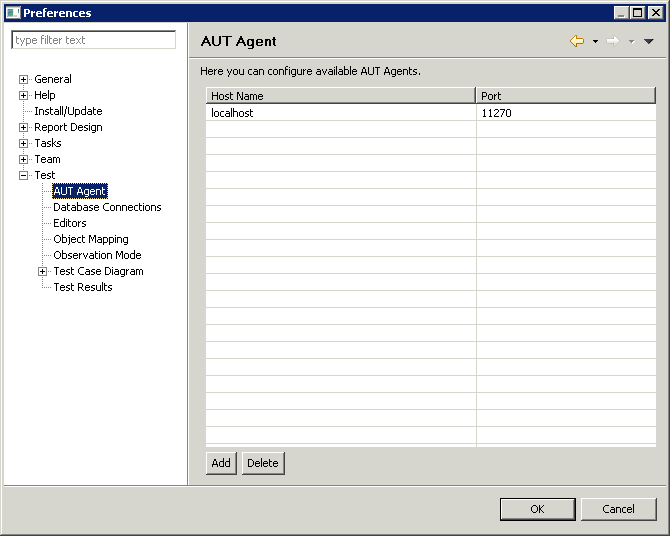
\includegraphics[width=12.5cm]{Tasks/Preferences/PS/serverconfig}
\caption{\gdagent Configuration Dialog}
\label{serverconfig}
\end{center}
\end{figure}










\subsection{Editor preferences}
\gdhelpid{editorPrefPageContextId}{Editor Preferences}
\index{Preferences!Editor}
\index{Editor!Preferences}
\label{editorprefs}

In the \bxname{Test - Editors} preferences, you can choose whether you want items (\gdcases{} and \gdsteps{}) to be placed at the bottom of the tree or after the selected item when you use the \bxname{add} option. 




\subsection{Object mapping preferences}
\gdhelpid{prefPageObjectMapContextId}{Object Mapping Preferences}
\label{TasksPrefsOMM}
% BREDEX LaTeX Template
%  \documentclass is either ``bxreport'' or ``bxarticle''
%                 option is bxpaper
%% \documentclass{bxarticle}
%% % ----------------------------------------------------------------------
%% \begin{document}
%% \title{}
%% \author{}
%% % \author*{Hauptautor}{Liste der Nebenautoren}
%% \maketitle
%% % ----------------------------------------------------------------------
%% \bxversion{0.1}
%% %\bxdocinfo{STATUS}{freigegeben durch}{freigegeben am}{Verteilerliste}
%% \bxdocinfo{DRAFT}{}{}{}
%% % ----------------------------------------------------------------------

%% \end{document}
\index{Preferences!Object Mapping}
\index{Object Mapping!Preferences}

\begin{figure}[h]
\begin{center}
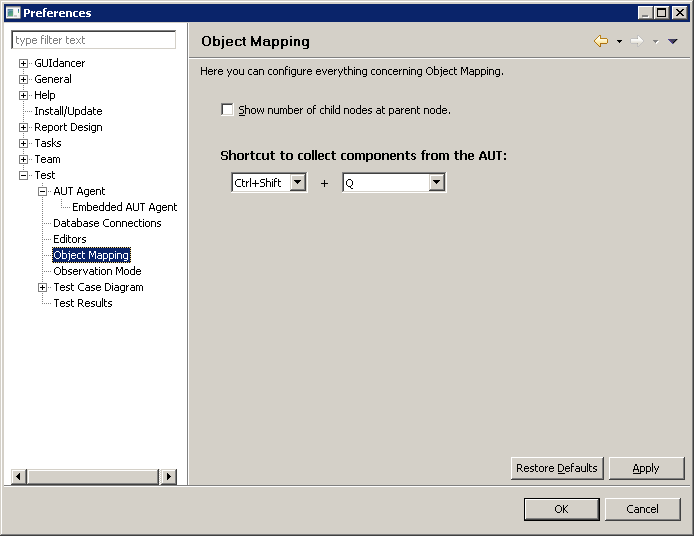
\includegraphics[width=12.5cm]{Tasks/Preferences/PS/objectmappingprefs}
\caption{Object Mapping Preference Dialog}
\label{objectmappingprefs}
\end{center}
\end{figure}

You can access the object mapping preferences from \bxname{Test - Object Mapping} in the preferences dialog. 
\begin{enumerate}
\item Select whether you want \app{} to display how many nodes are contained in each category in the \gdomeditor{}. 
\item Choose which keystrokes or mouse buttons you want to use to collect components in the \gdomm{}.  
\end{enumerate}

\bxtipp{If your \gdaut{} does not accept keystrokes, set the object collection preference to a mouse button combined with a modifier key.}


\subsection{Observation mode preferences}
\gdhelpid{prefPageObserveJavaContextId}{Observation Mode Preferences}
\label{TasksPrefsObsModeJava}
\index{Preferences!Observation Mode}
\index{Observation Mode!Preferences}

\bxtipp{The observation mode can only be used for Java \gdauts{}.}
\begin{description}
\item[Start/stop check mode:]{ Choose which keystroke you want to use to start and stop the check mode when you are observing \gdcases{} in Java \gdauts{}.}
\item [Check component:]{Choose which keystroke you want to use to show the check dialog when you are in check mode. The check dialog lets you choose what property of the selected component you want to check.}
\item [Show console:]{The console provides information on the actions that have been observed. This is especially useful if your \gdaut{} is running on a different machine to your client. }
\item [Trigger for replace text:]{Replace text actions are observed when the focus moves from the text component to another component. Depending on your application, this may not happen automatically in some situations. Enter triggers here which you can use to tell \app{} that you wish to observe a replace text action, even if the focus does not move from the text component. }
\end{description}

\begin{figure}[h]
\begin{center}
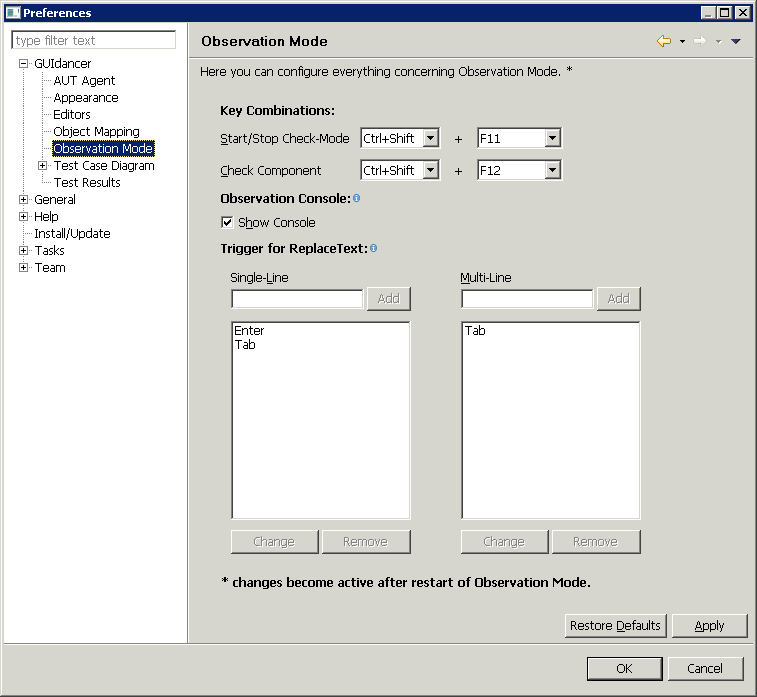
\includegraphics[width=0.60\textwidth]{Tasks/Preferences/PS/obsprefsjava}
\caption{Observation Mode Preference Dialog}
\label{obsprefsjava}
\end{center}
\end{figure}


%% \subsection{Observation mode preferences -- for Web}
%% \gdhelpid{prefPageObserveWebContextId}{Observation Mode Preferences}
%% \index{Preferences!Observation Mode Web}
\index{Observation Mode!Preferences}

On this preference page, you can configure the key combinations to observe normal actions and actions of the application component in the observation mode for web applications. 

\begin{figure}[h]
\begin{center}
\includegraphics[width=12.5cm]{Tasks/Preferences/PS/obsprefsweb}
\caption{Observation Mode for Web Preference Dialog}
\label{obsprefsweb}
\end{center}
\end{figure}



\subsection{\gdcase{} diagram preferences}
\gdhelpid{prefPageTCDGeneralContextId}{Test Case Diagram Preferences}
\label{TasksPrefsModel}
\index{Preferences!Test Case Diagram}
\index{Test Case Diagram!Preferences}

In the \gdcase{} diagram preferences page (\bxfigref{diagramprefs}), you can configure:

\begin{figure}[h]
\begin{center}
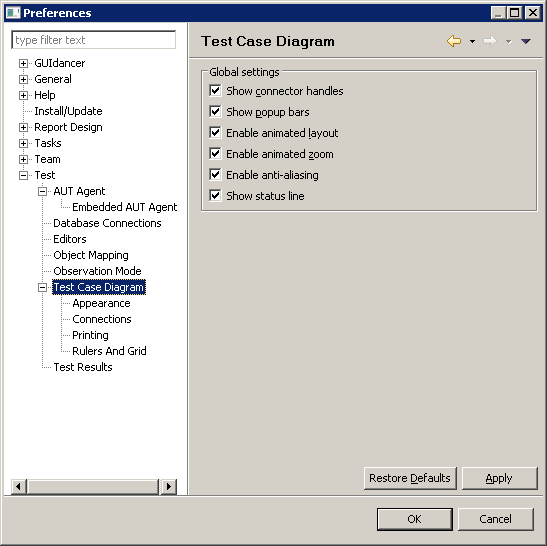
\includegraphics[width=12.5cm]{Tasks/Preferences/PS/diagramprefs}
\caption{Diagram Preference Dialog}
\label{diagramprefs}
\end{center}
\end{figure}

\begin{description}
\item [Connector handles:]{When this option is checked, you will see the connection arrows to add notes when an element is selected in your model. Click on a connector and drag to create a new note.}
\item [Pop up bars:]{When this option is checked, you will see a pop-up with the options to add parameters and \gdcase{} referenced when an element is selected in your model. Clicking on the \bxname{add parameter} or the \bxname{add \gdcase{} reference} icon will add the element you choose to the currently selected item. }
\item [Animated layout:]{When this option is activated, the arrangement of the items in the diagram will be animated when you click the \bxcaption{Arrange} button in the toolbar. }
\item [Animated zoom:]{When this option is activated, zooming into or out of the diagram will be animated. }
\item [Anti-aliasing:]{Use this option with higher-performance machines to smooth the lines connecting elements in the model. Machines with lower performance should deactivate this option. }
\end{description}

\subsubsection{\gdcase{} diagram appearance preferences}
\gdhelpid{prefPageTCDAppearanceContextId}{Test Case Diagram Appearance Preferences}
On the appearance preference page for the \gdcase{} diagram, you can specify which colors should be used within the model, for text and lines in the notes and in general. 

\begin{figure}[h]
\begin{center}
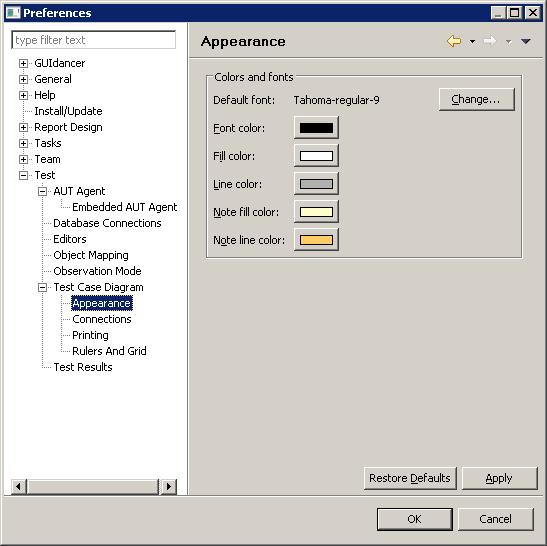
\includegraphics[width=12.5cm]{Tasks/Preferences/PS/diagramappearanceprefs}
\caption{Diagram Appearance Preference Dialog}
\label{diagramappearanceprefs}
\end{center}
\end{figure}

\subsubsection{\gdcase{} diagram connections preferences}
\gdhelpid{prefPageTCDConnectionsContextId}{Test Case Diagram Connections Preferences}
Use this preference page to specify how you would like the connections to appear in your model. 
\begin{description}
\item [Oblique]{displays the connectors as direct, straight lines between the connected elements. }
\item [Rectilinear]{displays connecting lines at right angles between the connected elements.}
\end{description}


\subsubsection{\gdcase{} diagram printing preferences}
\gdhelpid{prefPageTCDPrintingContextId}{Test Case Diagram Printing Preferences}
If you are planning on printing your \gdcase{} model, you can configure the print preferences in this page. For example, you can set the page orientation to portrait or landscape and use the context-sensitive menu in the model to view the page boundaries for your chosen orientation. 

\begin{figure}[h]
\begin{center}
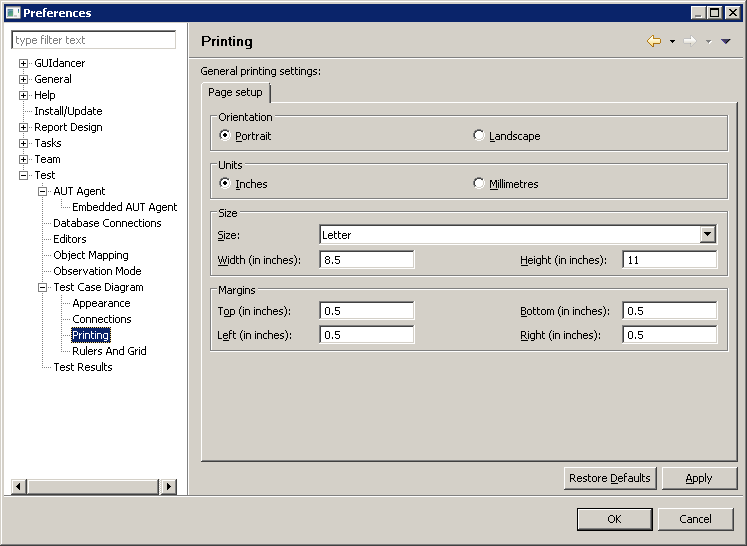
\includegraphics[width=12.5cm]{Tasks/Preferences/PS/diagramprintingprefs}
\caption{Diagram Printing Preference Dialog}
\label{diagramprintingprefs}
\end{center}
\end{figure}

\subsubsection{\gdcase{} diagram rulers and grid preferences}
\gdhelpid{prefPageTCDRulersContextId}{Test Case Diagram Rulers and Grid Preferences}
In this preference page, you can specify whether you want to see the rulers and the grid for new diagrams. In the ruler settings, you can also specify the ruler units as centimeters, inches or pixels. 

Within the grid options, you can choose whether elements should snap to the grid (\bxname{snap to grid}), or to each other (\bxname{snap to shape}). The snap to shape option displays a horizontal or vertical line when an element is moved close to another element. The line can be used to line elements up with each other. 

The grid spacing can also be altered to decrease or increase the size of the grid blocks.  

\begin{figure}[h]
\begin{center}
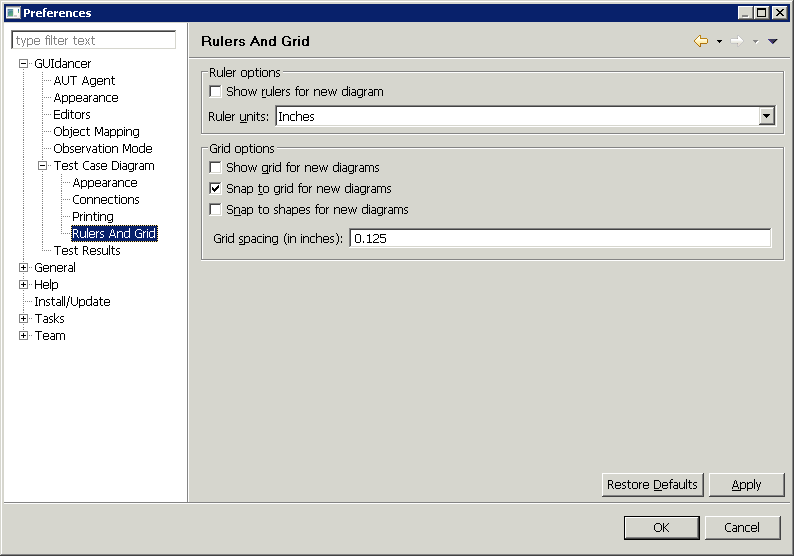
\includegraphics[width=12.5cm]{Tasks/Preferences/PS/diagramrulersprefs}
\caption{Diagram Rulers and Grids Preference Dialog}
\label{diagramrulersprefs}
\end{center}
\end{figure}


\subsection{Test result preferences}
\gdhelpid{prefPageTestResultContextId}{Test Result Preferences}
\label{testresprefs}
% $Id: testresultprefs.tex 12292 2010-09-23 12:45:32Z alexandra $
% Local Variables:
% ispell-check-comments: nil
% Local IspellDict: american
% End:
% --------------------------------------------------------
% User documentation
% copyright by BREDEX GmbH 2005
% --------------------------------------------------------
\index{Preferences!Test Result}
\index{Test Result!Preferences}
\index{XML and HTML Result Reports}
\index{Results!XML and HTML Reports}

You can open the test result preference page by selecting \bxname{Test - Test Results} from the preference dialog. 

\begin{figure}[h]
\begin{center}
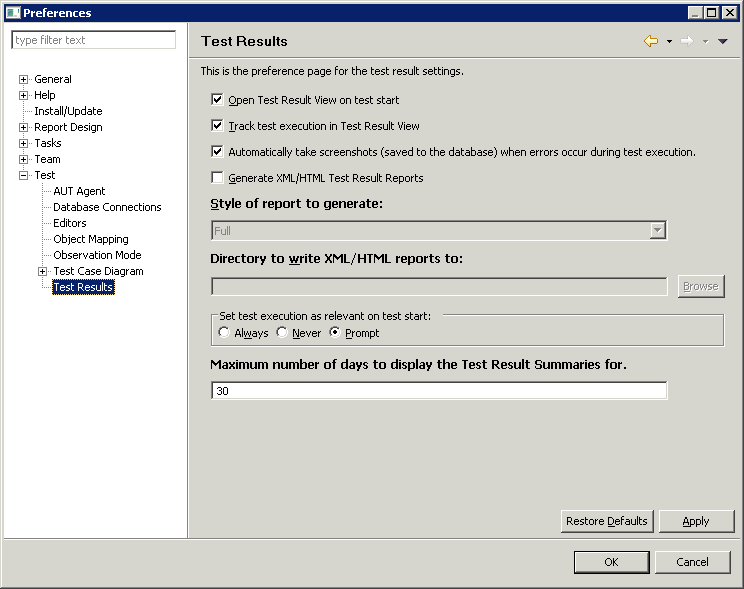
\includegraphics[width=0.6\textwidth]{Tasks/Preferences/PS/testresultprefs}
\caption{Test Result Preference Dialog}
\label{testresultprefs}
\end{center}
\end{figure}
\begin{enumerate}
\item Choose whether you want the  \gdtestresultview{} to open when testing begins. 

The \gdtestresultview{} follows the test execution and shows which \gdsteps{} were successful and which failed. 

\item Choose whether you want to track the test execution progress in the \gdtestresultview{}. When this option is activated, the \gdtestresultview{} scrolls to follow the test progress. 
\item Choose whether you want \app{} to automatically create a screenshot when a test encounters an error. Screenshots are automatically saved in the \gddb{} and can be viewed using the \gdimgview{} when you select the failed \gdstep{} in the \gdtestresultview{}. 
\item Choose whether you want to create HTML and XML reports for each execution. When you activate this choice, decide whether you want full reports or just the errors to be shown. Enter a directory for the reports. 
\item Decide whether you want all test runs or no test runs to be marked as relevant, or whether you want to be prompted each time. Non-relevant test results are not exported with the \gdproject{}. 
\item Enter the amount of days that test result summaries should be displayed for. This gives you a better overview of the most recent results in the \gdtestsummaryview{}. 
\end{enumerate}




\subsection{General/Keys preferences}
In the \bxname{General} preferences, you can select the \bxname{Keys} option to be able to edit the key binding for shortcuts in \jb{}. 


\subsection{Help preferences}
% $Id: helpprefs.tex 7847 2009-02-24 14:58:53Z alexandra $
% Local Variables:
% ispell-check-comments: nil
% Local IspellDict: american
% End:
% --------------------------------------------------------
% User documentation
% copyright by BREDEX GmbH 2005
% --------------------------------------------------------

\label{helpprefs}
\begin{enumerate}
\item Choose whether you want to have help displayed in an external browser. This lets you see more information at once. 
\item For context-sensitive help for windows and dialogs, choose how you want the help to appear. 
\item Choose how many search results should be shown when searching through the help system.  
\end{enumerate}

